% \documentclass[compacto,10pt]{aleph-notas}
\documentclass[compacto,5pt,comentarios]{aleph-notas}

% Se recomienda leer la documentación de esta
% clase en https://github.com/alephsub0/LaTeX_aleph-notas

% -- Paquetes adicionales
\usepackage{enumitem}
\usepackage{aleph-comandos}
\usepackage{float} % En el preámbulo
\usepackage{tcolorbox} % Paquete para tcolorbox
\usepackage{amssymb}   % Para el símbolo de check

% Nuevo entorno para Características
\newtheorem{carac}{Características}


% -- Datos del librod
\institucion{BSTAR 3D}
\carrera{Manufactura Aditiva \\}
\asignatura{Capacitación EPN \\ Impresión-Escaneo 3D}
\tema{Ing Mecatrónico - Área técnica}
\autor{Sebastián Osorio}
\fecha{20/11/2024}
\fuente{montserrat}

%% --> Logos de las guias
\logouno[4.5cm]{Logos/LogoBSTAR.jpeg}
\definecolor{colordef}{cmyk}{0.81,0.62,0.00,0.22}

\begin{document}

\encabezado

\section{Impresoras}




\subsection{Creality K1C}     

\begin{advertencia}
\begin{itemize}
    \item Hotend de 300° + boquilla de acero endurecido
    \item Velocidad máxima de 600mm/s
    \item Aceleración máxima 20000mm/s²
    \item Calibración automática
\end{itemize}
\end{advertencia}


\begin{figure}[h]
    \centering
    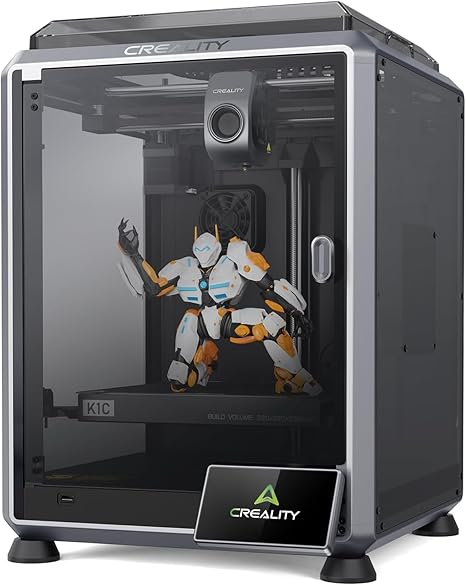
\includegraphics[width=0.5\linewidth]{Logos/K1C.jpg}
    %\caption{JAMG HE clear SG}
    \label{fig:enter-label}
\end{figure}

% Lorem ipsum dolor sit amet, consectetur adipiscing elit, sed do eiusmod tempor incididunt ut labore et dolore magna aliqua. Ut enim ad minim veniam, quis nostrud exercitation ullamco laboris nisi ut aliquip ex ea commodo consequat. Duis aute irure dolor in reprehenderit in voluptate velit esse cillum dolore eu fugiat nulla pariatur. Excepteur sint occaecat cupidatat non proident, sunt in culpa qui officia deserunt mollit anim id est laborum.

\begin{car}
\begin{itemize}
    \item Tecnología de impresión: FDM
    \item Volumen de impresión: 220*220*250 mm
    \item Dimensiones del producto: 358*374*498
    \item Nivelación automática:
    \item Pantalla: 4.3'' HD color táctil
    \item Peso neto: 7.83 kg
    \item Placa madre: 32-bit
    \item Compatible con: PLA, TPU, PETG, ABS, PLA-C, PETG-CF, CR-carbon
\end{itemize}
\end{car}
\begin{cont}
\begin{itemize}
    \item Impresora 3D Creality K1C (preensamblada en gran medida).
    \item Plataforma de impresión con superficie magnética.
    \item Fuente de alimentación integrada.
    \item Pantalla táctil a color.
    \item Bobina de filamento de muestra.
    \item Juego de herramientas básicas (llaves Allen, pinzas, cortador de filamento, aguja de limpieza).
    \item Cable de alimentación.
    \item Manual de usuario.
    \item Tarjeta microSD y lector USB.
\end{itemize}
\end{cont}
\begin{aplic}
\begin{itemize}
    \item Gama alta
    \item Prototipado rápido de alta precisión.
    \item Fabricación de piezas funcionales.
    \item Modelado industrial y diseño de productos.
    \item Investigación y desarrollo (I+D).
\end{itemize}
Diferenciación:
\begin{itemize}
    \item Alta velocidad de impresión.
    \item Mayor precisión y calidad en detalles.
    \item Capacidad para trabajar con materiales profesionales.
\end{itemize}
\end{aplic}


\newpage
\subsection{Creality Ender 3 V3}

\begin{advertencia}
\begin{itemize}
    \item Velocidad máxima de 600mm/s
    \item Aceleración máxima 20000mm/s²
    \item Calibración automática
\end{itemize}
\end{advertencia}

\begin{figure}[h]
    \centering
    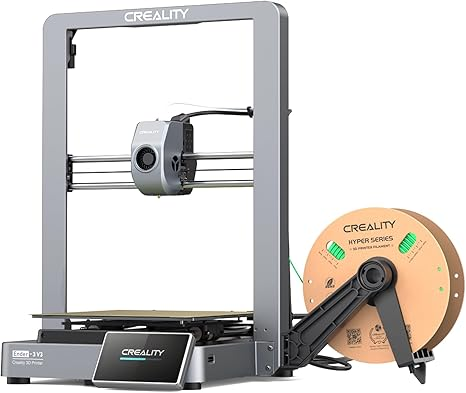
\includegraphics[width=0.5\linewidth]{Logos/Ender3V3.jpg}
    %\caption{JAMG HE clear SG}
    \label{fig:enter-label}
\end{figure}

\begin{car}
\begin{itemize}
    \item Tecnología de impresión: FDM
    \item Volumen de impresión: 220*220*250 mm
    \item Dimensiones del producto: 358*374*498
    \item Nivelación automática: Sí
    \item Pantalla: 4.3'' HD color táctil
    \item Peso neto: 7.83 kg
    \item Placa madre: 32-bit
    \item Compatible con: PLA, TPU, PETG, ABS, PLA-C, PETG-CF, CR-carbon
\end{itemize}
\end{car}
\begin{cont}
\begin{itemize}
    \item Marco principal de la impresora (parcialmente ensamblado).
    \item Plataforma de impresión con superficie de vidrio o magnética.
    \item Pantalla LCD con perilla de control.
    \item Fuente de alimentación externa.
    \item Bobina de filamento de muestra.
    \item Juego de herramientas (llaves Allen, destornillador, pinzas, aguja de limpieza).
    \item Espátula para retirar impresiones.
    \item Cable de alimentación.
    \item Manual de ensamblaje y uso.
    \item Tarjeta microSD y lector USB.
\end{itemize}
\end{cont}

\begin{aplic}
\begin{itemize}
    \item Gama: Media
\item Prototipado de modelos funcionales intermedios.
\item Uso educativo para enseñanza de impresión 3D.
\item Proyectos personales y hobbies.
\item Creación de accesorios y gadgets simples.
\end{itemize}

Diferenciación:
\begin{itemize}
    \item Adecuada para proyectos intermedios.
    \item Amplia comunidad de usuarios y soporte.
\end{itemize}

\end{aplic}

\newpage
\subsection{Voxelab Aquila S3}
\begin{advertencia}
\begin{itemize}
    \item Velocidad máxima de 200mm/s
    \item Cama de PEI texturizado
    \item Calibración automática
\end{itemize}
\end{advertencia}

\begin{figure}[h]
    \centering
    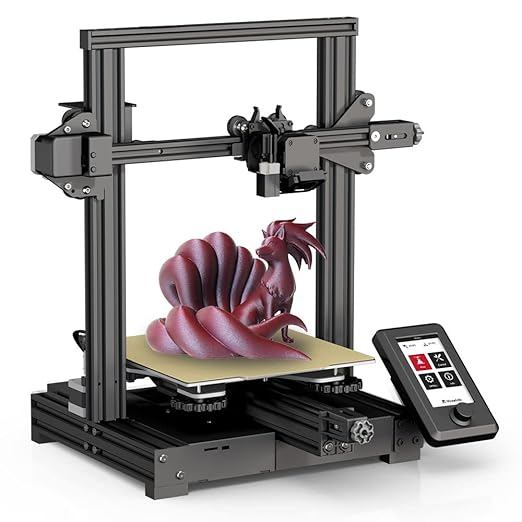
\includegraphics[width=0.5\linewidth]{Logos/AquilaS3.jpg}
    %\caption{JAMG HE clear SG}
    \label{fig:enter-label}
\end{figure}

% Lorem ipsum dolor sit amet, consectetur adipiscing elit, sed do eiusmod tempor incididunt ut labore et dolore magna aliqua. Ut enim ad minim veniam, quis nostrud exercitation ullamco laboris nisi ut aliquip ex ea commodo consequat. Duis aute irure dolor in reprehenderit in voluptate velit esse cillum dolore eu fugiat nulla pariatur. Excepteur sint occaecat cupidatat non proident, sunt in culpa qui officia deserunt mollit anim id est laborum.

\begin{car}
\begin{itemize}
    \item Tecnología de impresión: FDM
    \item Volumen de impresión: 220*220*240 mm
    \item Dimensiones del producto: 480*473*473
    \item Nivelación automática: Sí, 25 puntos
    \item Pantalla electronica a color
    \item Peso neto: 7.9 kg
    \item Placa madre: 32-bit
    \item Compatible con: ABS, PETG, PA, PLA, TPU y madera
\end{itemize}
\end{car}
\begin{cont}
\begin{itemize}
    \item Estructura principal de la impresora (kit semidesarmado).
    \item Plataforma de impresión de vidrio.
    \item Pantalla táctil o LCD estándar con perilla.
    \item Fuente de alimentación.
    \item Bobina de filamento de muestra.
    \item Juego de herramientas (llaves Allen, pinzas, cortador de filamento).
    \item Cable de alimentación.
    \item Manual de ensamblaje y guía de inicio rápido.
    \item Tarjeta microSD y adaptador USB.
\end{itemize}
\end{cont}
\begin{aplic}
\begin{itemize}
    \item Gama: Media-Baja
    \item Prototipos y modelos funcionales sencillos.
    \item Proyectos de aficionados y makers.
    \item Impresión educativa.
\end{itemize}
Diferenciación:
\begin{itemize}
    \item Precio accesible.
    \item Buen rendimiento para iniciados y proyectos sencillos.
    \item Resolución y precisión menores que modelos de gama media o alta.
\end{itemize}



\end{aplic}



\newpage
\section{Configuración y preparación de impresoras 3D}
\begin{itemize}
    \item \textbf{Instalación inicial:} Configuración básica del firmware y conexiones.
    \item \textbf{Nivelación de la cama:} Manual o automática según modelo, esencial para adherencia.
    \item \textbf{Calibración:} Ajuste de ejes XYZ y extrusión para precisión.
    \item \textbf{Materiales:} Uso de filamentos como ABS y PLA, con sus ventajas (resistencia vs facilidad).
    \item \textbf{Mantenimiento:} Limpieza regular de boquillas y engranajes para evitar fallas.
\end{itemize}

\section{Software de impresión 3D}
\begin{itemize}
    \item \textbf{Programas de slicing:} Generación de instrucciones G-code a partir de modelos 3D.
    \item \textbf{Configuración:} Ajuste de parámetros según impresora (altura de capa, velocidad).
    \item \textbf{Manipulación de modelos:} Escalado, rotación y corte previo a impresión.
    \item \textbf{Slicers destacados:}
    \begin{itemize}
        \item \textbf{Orca Slicer:} Optimizado para impresiones detalladas.
        \item \textbf{Cura:} Intuitivo, gran compatibilidad.
        \item \textbf{Prusa Slicer:} Enfoque en modelos avanzados y configuraciones personalizadas.
    \end{itemize}
\end{itemize}

\section{Proceso de impresión 3D}
\begin{itemize}
    \item \textbf{Inicio:} Verificación de configuración previa, pre-calentamiento.
    \item \textbf{Problemas comunes:} Warping, atascos; soluciones prácticas.
    \item \textbf{Extracción del modelo:} Uso de herramientas adecuadas para evitar daños.
    \item \textbf{Revisión de fallas:} Inspección visual y ajustes en parámetros de impresión.
\end{itemize}

\newpage
\section{Escáner Shinning Einstar} 

\begin{advertencia}
\begin{itemize}
    \item Alta fidelidad de color
    \item Datos de alta calidad (0.10 mm)
    \item Cómodo para los ojos
    \item Fácil de escanear el cabello
\end{itemize}
\end{advertencia}

\begin{figure}[H]
    \centering
    \begin{minipage}[t]{0.48\linewidth}
        \centering
        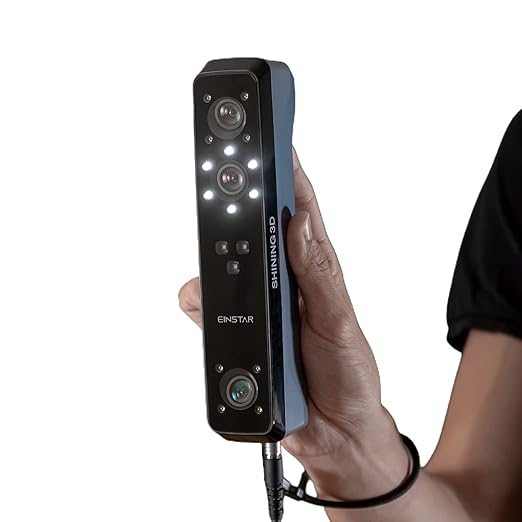
\includegraphics[width=\linewidth]{Logos/Einstar.jpg}
        \caption{Referencia del escáner \\ Einstar}
        \label{fig:imagen1}
    \end{minipage}%
    \hfill
    \begin{minipage}[t]{0.48\linewidth}
        \centering
        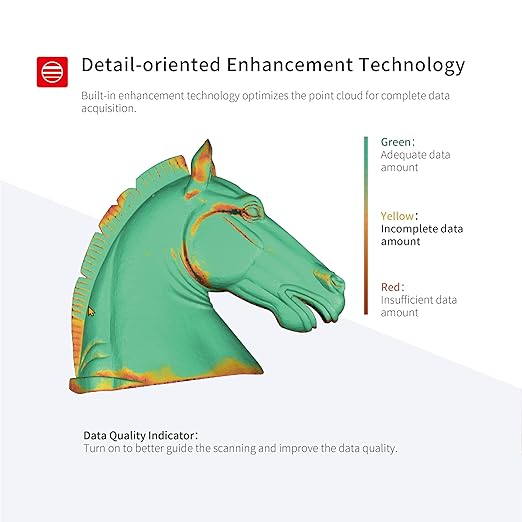
\includegraphics[width=\linewidth]{Logos/Einstar_Details.jpg}
        \caption{Tecnología de calidad \\ de datos}
        \label{fig:imagen2}
    \end{minipage}
    %\caption{Ambas imágenes lado a lado}
    \label{fig:dos-imagenes}
\end{figure}

Einstar se utiliza en impresión 3D, diseño, archivo digital, educación, cultura y arte, VR y AR.

\textit{\textbf{¿Qué tamaño de objeto puede escanearse con mayor o menor tamaño?}}

La medida más reducida recomendada es 100*100*100 mm. La mayor dimensión depende de la RAM; una RAM más amplia puede alojar objetos de mayor tamaño.

\textbf{\textit{¿Por qué optar por el escáner Einstar en 3D?}}

Einstar proporciona una mayor visión con un campo de visión más extenso, lo que simplifica considerablemente ciertos trabajos complicados como el escaneo de colores oscuros, cabello y áreas exteriores. El programa que permite un seguimiento inteligente, alineación automática y una fácil edición de datos contribuye a regular la calidad de la información. El escáner y el software resultan más sencillos y muy intuitivos para los usuarios, incluso si es su primera experiencia con el escaneo en 3D.


% Lorem ipsum dolor sit amet, consectetur adipiscing elit, sed do eiusmod tempor incididunt ut labore et dolore magna aliqua. Ut enim ad minim veniam, quis nostrud exercitation ullamco laboris nisi ut aliquip ex ea commodo consequat. Duis aute irure dolor in reprehenderit in voluptate velit esse cillum dolore eu fugiat nulla pariatur. Excepteur sint occaecat cupidatat non proident, sunt in culpa qui officia deserunt mollit anim id est laborum.

\begin{car}
\begin{itemize}
    \item Tecnología de impresión: FDM
    \item Volumen de impresión: 220*220*250 mm
    \item Dimensiones del producto: 358*374*498
    \item Nivelación automática:
    \item Pantalla: 4.3'' HD color táctil
    \item Peso neto: 7.83 kg
    \item Placa madre: 32-bit
    \item Compatible con: PLA, TPU, PETG, ABS, PLA-C, PETG-CF, CR-carbon
\end{itemize}
\end{car}

\begin{cont}
\begin{itemize}
    \item Escáner 3D Einstar
    \item Estuche de transporte ligero
    \item Estuche de silicona y correa de transporte
    \item Guía introductoria del usuario
    \item Marcadores de posicionamiento
    \item Paño para limpiar la lente
    \item Fuente de alimentación y cable USB
\end{itemize}
\end{cont}
\end{document}